\documentclass[tikz]{standalone}
\usepackage{fontspec}
\renewcommand*{\familydefault}{\sfdefault}
\usepackage{standalone}
\usepackage{amssymb}
\usetikzlibrary{positioning, arrows.meta, decorations.pathreplacing, shapes.geometric}
\usetikzlibrary{er}
%\usetikzlibrary{positioning,fit,shapes.geometric,fadings,bayesnet}

\begin{document}

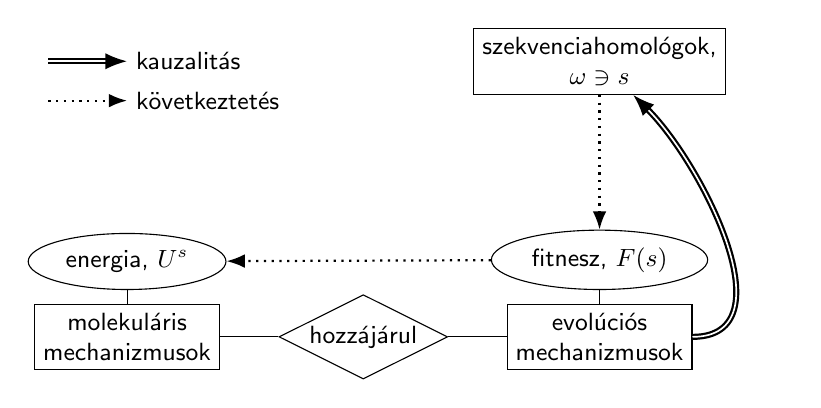
\begin{tikzpicture}[every relationship/.style={aspect=2.0}]
\small
\path
(0,0) node[entity, align=center] (seq-hom) {szekvenciahomológok,\\ \(\omega\ni s\)}
++(-90:3.5 cm) node[entity, align=center] (evol-mech) {evolúciós \\ mechanizmusok}
node[attribute] (F) [above=5 pt of evol-mech] {fitnesz, \(F(s)\)}
++(180:3.0 cm) node[relationship, align=center] (contrib) {hozzájárul}
++(180:3.0 cm) node[entity, align=center] (mol-mech) {molekuláris \\ mechanizmusok}
node[attribute] (U) [above=5 pt of mol-mech] {energia, \(U^s\)}
++(90:3 cm) coordinate (a0) +(180:1 cm) coordinate (a1)
+ (0:0.0 cm) node[anchor=west] {következtetés}
++(90:0.5 cm) coordinate (b0) +(180:1 cm) coordinate (b1)
+ (0:0.0 cm) node[anchor=west] {kauzalitás}
;


\draw (mol-mech) -- (U) ;
\draw (evol-mech) -- (F) ;

\draw[thick, dotted, -Latex] (a1) -- (a0) ;
\draw[thick, double, -Latex] (b1) -- (b0) ;

\draw[]
(mol-mech) -- (contrib) -- (evol-mech)
;

\draw[thick, double, -Latex]
(evol-mech.east) to[out=0, in=-45] (seq-hom)
;

\draw[thick, dotted, -Latex]
%(seq-hom) -- (U)
(seq-hom) -- (F) 
;

\draw[thick, dotted, -Latex]
(F) -- (U)
;

\end{tikzpicture}

\end{document}
